% 原书第 347 页（PDF 第 360 页）
\BookPage{347}{360}
\BookHeading{红票：一封康熙皇帝寄给罗马教皇的信}{红票：一封康熙皇帝寄罗马教廷的信}{冯明珠*}
<红票〉、〈红字票〉或译称〈红色谕旨〉的清代档案，是康熙皇帝传谕十六位西洋传教士署名，发给所有来华即将返航的西洋人士，嘱他们带回大西洋（欧洲)转交罗马教廷的一封公开信。我注意到这件档案始于2002年，当时我正利用国立故宫博物院（以下简称故宫）所藏《康熙与罗马使节关系文书》与康熙朝满汉文朱批奏折撰写〈坚持与容忍一档案中所见康熙皇帝对中梵关系生变的因应〉1，在方豪师撰《中国天主教史人物传》〈艾若瑟〉²条中读到了这件档案:「在罗马传信部档案处东方文献第十三卷内，藏有伊都立等告西洋人书，系康熙五十五（1716）年九月十七日发，木刻，满文、拉丁文对照，在拉丁文后有十六位供职内廷洋人署名，最后一位是郎世宁。档案内文，〈艾若瑟〉小传中已有节录，但档案的外型究竟如何？属于那类文种？则是我所关切的。很幸运在2007年北京故宫召开的「第一届清宫典籍国际学术研讨会」中，终于看到了〈红票〉的影像，特向大会索取作为教学之用。两年前故宫策划「康熙大帝与太阳王路易十四一中法艺术文化的交会特展」，本人建议向法国国家图书馆借展红票〉，终于成事，得以近观真迹。本文旨在介绍档案及档案背后蕴含的历史事件及清圣祖康熙皇帝在处理中梵交涉中展现的惊人耐心与心胸。

\BookSubheading{一、红票}

〈红票〉清代官员称为〈红字票〉，「康熙大帝与太阳王路易十四特展」3中根

\vfill
\begin{BookNotes}
\BookNote{*}{作者任职于国立故宫博物院。}
\BookNote{1.}{发表于《中梵外交关系史国际学术研讨会论集》，辅仁大学历史系印行，2002年12月。}
\BookNote{2.}{方豪《中国天主教史人物传》第三册，页30-31〈艾若瑟〉，香港公教真理学会出版，1970年。}
\BookNote{3.}{「康熙大帝与太阳王路易十四—中法艺术文化的交会特展由国立故宫博物院主办，展期2011年10月3日至2012年1月3日。}
\end{BookNotes}

% 原书第 348 页（PDF 第 361 页）
\BookPage{348}{361}
\noindent 据法文Le Décret rouge译作〈红色谕旨〉，是一张纵48.4公分、横95.5公分，木刻朱印纸本公文书，文书分三部分，中间由右到左直排汉文，左边由左到右直行满文，右侧由左到右横书拉丁文，拉丁文下刻有十六位传教士的签名，四周饰以「行龙追日」纹饰，就文件外型论与明代的〈龙边敕谕〉相似；然就文件启首用语与内容格式论，它不是一件〈敕谕〉4，而是由武英殿监修书官伊都立（?-1753）、王道化（生卒不详）、赵昌（1657-1731）等发出的〈寄信上谕〉（又称廷寄），收信者是「自西洋来的众人」，嘱他们将〈红票〉带回大西洋（欧洲）去。这件〈寄西洋众人谕〉汉文全文如下：

\begin{BookQuote}
武英殿等处监修书官伊都立、王道化、赵昌等字寄与自西洋来的众人:我等谨遵旨于康熙四十五年已曾差西洋人龙安国、薄贤士；四十七年，差西洋人艾若瑟、陆若瑟奉旨往西洋去了。至今数年，不但没有信来，所以难辨真假。又有乱来之信，因此与鄂罗斯的人，又带信去，想是到去了。必竟我等差去人回时，事情都明白之后，方可信得。若是我等差去之人不回，无真凭据，虽有甚么书信，总信不得。因此唯恐书信不通，写此字兼上西洋字刊刻，用广东巡抚院印，书不封缄，凡来的众西洋人，多发与带去。康熙五十五年九月十七日。
\end{BookQuote}

(图一)

\BookArt{p361-01.jpg}{0.990}{0.332}

\vfill
\begin{BookNotes}
\BookNote{4.}{敕谕〉启首句当为：「奉天承运，皇帝制曰」。}
\end{BookNotes}

% 原图说　图一　〈红票〉又称〈红字票〉，法国国家图书馆称为 Le Décret rouge，译作〈红色谕旨〉，经语文专家校阅档案中满文及拉丁文内容与汉文相同。这件档案在欧洲书馆典藏普遍，本文影像来自法国国家图书馆收藏。

% 原书第 349 页（PDF 第 362 页）
\BookPage{349}{362}
\noindent 根据两广总督杨琳（？-1724）奏称，他于康熙五十五年（1716）十月接到伊都立等奉旨发来的〈红票〉，立即盖上巡抚官防，发与所有出洋船只上较体面的人带回西洋去了。故宫藏有康熙皇帝御批〈红票〉汉文底稿（图二），详后文。

\BookArt{p362-01.jpg}{0.570}{0.269}

\BookArt{p362-02.jpg}{0.461}{0.075}

康熙皇帝究竟为何事发出这道〈廷寄〉?〈廷寄〉中所言:康熙四十五年(1706）差西洋人龙安国（Antoniusde Burros,1664-1708）与薄贤士（Antoine de Beanvollier,1656-1708）；四十七年（1708)，差西洋人艾若瑟（Joseph-Antoine Provana,1662-1720）、陆若瑟（Raymond-Joseph Arxo,1659-1711）前往西洋所为何事？康熙皇帝在等什么信讯？这道〈廷寄〉究竟有没有发挥功能？这是本文介绍重点之一。

\BookSubheading{二、颁谕背景一礼仪之争与多罗使华}

颁发〈红票〉与中梵关系史中的「礼仪之争」有关。诚如大家所知，康熙三十二年（1693）三月间，接任福建地区宗座代牧主教的巴黎外方传教会会士严珰（亦译作阎珰或颜珰Charles Maigrot,1652-1730）引爆了「礼仪之争」，严珰改变了耶稣会士利玛窦（MatteoRicci,1552-1610）一百多年来⁵尊重中国礼俗的宣教传统，不但要求在华西洋传教士向他宣誓服从，并发布「主教通谕」，禁止天主教徒参与敬天、尊孔、祭祖等活动，并呈请教廷宣布全面实施，引起康熙三十八至四十三年（1699-1704）间罗马教廷有关中国礼仪的审查辩论，促使教廷注意中国教区问题，正式遣使

\vfill
\begin{BookNotes}
\BookNote{5.}{自1583年利玛窦到达中国至1705年教廷发布〈禁约〉前后一百多年。}
\end{BookNotes}

% 原图说　图二　康熙御批〈红票〉底稿　《康熙与罗马使节关系文书》文献编号802000016　国立故宫博物院藏
% 原图说　该档案所载内容几乎与〈红票〉（图一）汉文全同

% 原书第 350 页（PDF 第 363 页）
\BookPage{350}{363}
\noindent 来华。康熙四十一年，罗马教皇克莱门十一世（Clement XI，1649-1721）为了落实教权及解决教务纷争，派特使多罗(CarloTommaso Maillard deTournon,1668-1710)出使中国，谒见康熙皇帝。

多罗于康熙四十四年（1705）年搭乘法王路易十四的船只，经印度、马尼拉等地抵达澳门，六月初八日批准进京，十一月初七日抵达北京，十一月二十日康熙皇帝接见了多罗，觐见时多罗表示此行目的为：

\begin{BookQuote}
来中国之西洋教徒，蒙圣主体恤施恩，教化王（教皇）闻之感戴皇恩，特派我谢，此外并无他事。7
\end{BookQuote}

全然未提到礼仪问题。到了康熙四十五年三月间，多罗得到从马尼拉转来教廷作出禁止中国礼仪的讯息（教廷于1705年11月20日发布），态度转强，停止北京耶稣会士及天主教徒间有关礼仪问题的讨论、陈情与请愿，贯彻执行教廷禁令，并传唤严珰到北京，助他向康熙皇帝阐明禁止中国礼仪的道理。就在严珰到京至多罗离京之间，满文朱批奏折〉中出现了好几则康熙皇帝派武英殿总监造赫世亨（1648-？）与赵昌等传达他对教廷〈禁约〉的看法，并反复用各种有趣而浅显的比喻说明敬天、祭祖、尊孔等中国礼仪与天主教信仰无涉，实不必禁止。赫世亨与赵昌奔走于康熙与多罗之间，负责传旨及观察多罗等的反应与动静，随时向康熙皇帝回报；透过这些报告可以了解康熙皇帝的立场，并看到多罗对康熙传谕的回应，更可说明康熙皇帝在礼仪问题争辩中曾做过的努力。

康熙四十五年五月底，康熙皇帝与多罗间因礼仪问题形成僵局，多罗欲离京，康熙则令多罗将其旨意写成书信，待钦定后寄与教皇；康熙又令严珰将「中国礼仪」与天主教教义不合之处尽量写出呈览。例如，五月二十五日，康熙令赫世亨与赵昌向多罗传谕：

\begin{BookQuote}
中国行礼于牌，并非向牌求福禄，盖以敬礼而已。此乃中国之一要典，关系甚
\end{BookQuote}

\vfill
\begin{BookNotes}
\BookNote{6.}{案：本文配合档案，以农历系时，唯征引史籍原载为阳历时，则换算为农历，以求行文划一。}
\BookNote{7.}{详方豪《中国天主教史人物传》第二册，页313-325〈多罗〉。康熙45年7月10日〈武英殿总监赫世亨等奏报诘问西洋人多罗情形折〉(详附表）。}
\BookNote{8.}{方豪《中国天主教史人物传》第二册，页313-325，〈多罗〉；第三册，页21-26，〈阎珰〉。}
\end{BookNotes}

% 原书第 351 页（PDF 第 364 页）
\BookPage{351}{364}
\begin{BookQuote}
巨。…譬如以御用之履赐尔赵昌，尔必以贵物珍藏，尔岂敬朕之履耶？盖念朕所赐，故敬之矣。岂可向履求幸福？…多罗恭赉朕赏物到西洋后，必举之敬告皇上所赐者。多罗敬此物，岂向此物求幸福耶？亦念朕所赐之物，自然崇敬
\end{BookQuote}

之。9

这两则浅白的举例，目的是向多罗说明中国人施礼于牌位，并非宗教迷信，而是追忆先人的方法与反应。康熙并令赵昌以自身为例向严珰等说明中、西礼俗相异，不宜强同的道理。于是赵昌向严珰等说：

\begin{BookQuote}
西洋例娶一妻，今我有二、三妻，皆已生子，今我岂弃此妻子耶？奈何？10
\end{BookQuote}

据方豪考证，赵昌为康熙最亲信之内侍，随侍康熙五十余年，凡涉西洋之事多令赵昌处理；赵昌也因与西洋传教士相处日久，受感召而欲入教，但因有妾而未能领洗。11又据陈国栋〈养心殿总监造赵昌一为康熙皇帝照顾西洋人的内务府成员之一〉一文，赵昌于康熙驾崩后，即被抄家入狱，姬妾散尽，孑然一身后，于雍正九年夏受洗成为天主教徒。12

被召唤入京，协助多罗向康熙皇帝阐明教禁的严珰，康熙皇帝一再传谕令他将「孔子之道与天主之道不符之处」解说明白，却发现严珰根本不识中国字；热河行宫御座后「敬天法祖」匾额四字，竟只认得「天」字，更遑论中国哲理。13康熙气愤传谕：「譬如立于大门之前，论人屋内事，众人何以服。」14（图三）严珰的一名通译名叫陈修，是个汉人，从小由教堂养大，虽识字能写，但不通文理，自然也写不出康熙

\vfill
\begin{BookNotes}
\BookNote{9.}{引自康熙45年7月27日武英殿总监赫世亨、赵昌等〈奏报西洋人情形折〉。}
\BookNote{10.}{同上。}
\BookNote{11.}{详方豪〈清代旗人之信奉天主教与遭禁〉，《故宫文献》，第四卷第四期，页1-23，国立故宫博物院，1973年9月。}
\BookNote{12.}{详陈国栋〈养心殿总监造赵昌一为康熙皇帝照顾西洋人的内务府成员之一〉，《故宫文物月刊》343期，页44-51，国立故宫博物院，2011年10月；又见本辑〈康熙小臣养心殿总监造赵昌生平小考页269-310。}
\BookNote{13.}{案当康熙皇帝在热河行宫召见严珰时，发现他对御座后匾额上「敬天法祖」四字，只认识「天」字。详方豪《中国天主教史人物传》第三册，页21-26，〈阎珰〉及罗光《教廷与中国使节史》页116-117，台北：传记文学出版社，1983年。}
\BookNote{14.}{《康熙与罗马使节关系文书》802000014，国立故宫博物院藏。}
\end{BookNotes}

% 原书第 352 页（PDF 第 365 页）
\BookPage{352}{365}
\BookArt{p365-01.jpg}{0.842}{0.411}

\noindent 皇帝要求的道理里。15六月十三日，康熙再令赵昌等传谕多罗:「中国人绘神时画云云，西洋人画神添翼」，「云」与「翼」仅达意方式不同，如「天主」与「敬天」的差别，其象征意义是相同的。严珰向教徒宣布的七项禁令中，禁止教徒用「天」和「上帝」，概以「天主」替代。恰巧多罗使团中有名「毕天祥」(Ludovicus-Antonius Appiani,1663-1732）担任翻译者，康熙皇帝便以「毕天祥」为例，诘问何不改名「毕天主慈祥」?并进一步阐释:「各国起名，皆遵本国语法，岂以名词之故，便言大不同乎？」16康熙曾赐给北京天主堂「敬天」匾额，康熙解释此非「苍苍有形之天」，，乃「天地万物根源的主宰」17。

根据赵昌等奏报，多罗每次聆听传达康熙旨意时，态度虽然恭谨，意志却十分坚定，以致被赵昌等形容:「明知已非，断不认错」。18总之，这是一次没有交集而

\vfill
\begin{BookNotes}
\BookNote{15.}{康熙45年5月27日武英殿总监造赫世亨、赵昌〈奏报西洋人情形〉及康熙45年6月7日〈奏报西洋人情形〉}
\BookNote{16.}{康熙45年6月13日武英殿总监造赫世亨、赵昌〈奏报西洋人传宣谕旨折〉。}
\BookNote{17.}{方豪《中国天主教史人物传》第二册，〈多罗〉，页317。}
\BookNote{18.}{康熙45年7月10日武英殿监造赫世亨、赵昌等〈奏报西洋人情形折〉。}
\end{BookNotes}

% 原图说　图三　〈传谕多罗〉　《康熙与罗马使节关系文书》文献编号802000014　国立故宫博物院藏

% 原书第 353 页（PDF 第 366 页）
\BookPage{353}{366}
\noindent 各有坚持的交流，多罗于康熙四十五年九月离开北京，前往继续行使他奉命来华的职责，十二月二十二日，在南京正式发布教廷〈禁约〉：

\begin{BookQuote}
不许（天主教徒）祭孔、祭天，不许供牌位，不许以天或上帝称天主，不遵守的，即应受「弃绝」（excommunication）重罚。教宗与特使保留赦免权。19
\end{BookQuote}

康熙皇帝也探取宣示教权的做法，下令逮捕毕天祥，驱逐严珰，并传谕：

\begin{BookQuote}
凡不回去的西洋人等，写票用内务府印给发，票上写西洋某国人，年若干，在某会，来中国若干年，永不复回西洋，已经来朝觐陛见，为此给票。兼满汉字，将千字文编成号数，挨次存记，将票书成款式进呈。钦此。20
\end{BookQuote}

据康熙四十五年十二月二十五日所发「元字号票」21，传教必先领票，领票必须陛见，并表达永远居留中国的意愿，无疑是向康熙皇帝宣誓效忠，成为中国子民，自当遵守清廷「法度」，这正是康熙皇帝宣示教权的一种做法。22（图+二）康熙四十六年二月，康熙皇帝六度南巡，在临清、扬州、南京、苏州、杭州等处接见了传教士，凡不愿领票者，一律解送广州天主堂居住，多罗则逐居澳门。23

三红色谕旨

在康熙皇帝初次接见多罗的两天后（康熙四十四年十一月二十六日），康熙便准备派法国耶稣会士白晋（JoachimBouvet，1656-1730）、沙国安（Mariani）为正、副

\vfill
\begin{BookNotes}
\BookNote{19.}{引自方豪《中国天主教史人物传》第二册，页325，全文中译内容则详见于顾卫民《中国与罗马教廷关系史略》（北京东方出版社，2009年9月），页69-71；顾氏引自RayR.Nou,100 Roman Documents ConcerningtheChinese Rites Controversy (1645-1914)将该函公布时间系于阳历1707年1月25日，故本顾氏系年，唯配合本文系时，将阳历转为农历。}
\BookNote{20.}{见方豪《中国天主教史人物传》第二册，页324；第三册，页19-20〈毕天祥〉及页21-26〈严珰〉。}
\BookNote{21.}{见〈清宫画家郎世宁年谱一兼在华耶稣会士史事稽年〉（《故宫博物院院刊》1988年第二期，北京：故宫博物院）及高振田〈康熙帝与西洋传教士〉（《明清档案与历史研究》1986年第一期，北京：第一历史档案馆），康熙45年12月开始发票，47年对领票及未领票的西洋人进行查核，未领者解送澳门，驱逐出国。「元字号」票图像，见前引文。}
\BookNote{22.}{案若细读《康熙与罗马使节关系文书》〈谕孟由义等众西洋人〉802000002，则更可见发生在中国的皇权与教权之争，在华传教士实左右为难，最后康熙皇帝安慰领过票的人说：「你们领过票，就如中国人一样，尔等放心，不要害怕领票」。}
\BookNote{23.}{见方豪《中国天主教史人物传》第二册，页325。}
\end{BookNotes}

% 原书第 354 页（PDF 第 367 页）
\BookPage{354}{367}
\par\addvspace{4pt}\noindent
\begin{minipage}[t]{0.346\linewidth}
\vspace{0pt}
\noindent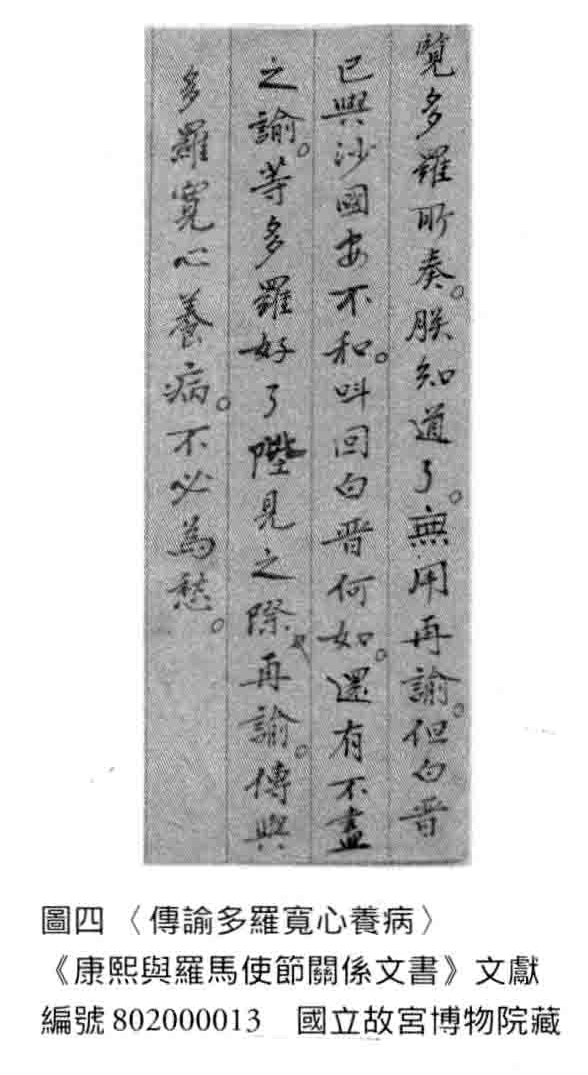
\includegraphics[width=\linewidth,height=.81\textheight,keepaspectratio]{assets/p367-01.jpg}
\end{minipage}
\hfill%
\begin{minipage}[t]{0.629\linewidth}
\vspace{0pt}\setlength{\parindent}{1.5em}
\noindent 使回聘教廷，但因多罗反对以白晋为首而作罢。24（图四)其后在礼仪问题争论不休时，康熙开始怀疑多罗的顽固究竟是教皇的意思或是多罗已见呢？于是又引发康熙遣使回聘教廷的想法，他要向教皇直接说明「中国礼仪」问题，并将多罗等破坏利玛窦尊重中国礼俗的传教方式晓谕教廷。康熙四十五年九月初，多罗已离京南下，康熙决定派龙安国与薄贤士带着他的敕谕前往教廷。薄贤士通汉文，多罗来京期间，康熙曾将薄贤士所撰汉字书三篇赠与多罗。25九月初六日，当薄贤士接获奉使消息，他向康熙表达：我来京城，未为皇上效力，而蒙格外抬举，视为可信之人，委以官差。…我当尽心竭力，将御诏送达。

\end{minipage}
\par\addvspace{4pt}

\noindent 遂于九月十日离京。26康熙皇帝令薄贤士奉往教廷〈御诏〉的具体内容为何？已不可考，但不外呼是谕教廷遵循利玛窦规矩传教。27到了康熙四十六年二月，康熙获得由闵明鄂（Claudio FilippoGrimaldi,1638-1712）传来的消息，薄贤士与龙安国已于去年十一月三十日乘船出洋，十二月初三日至海口，初四日前往西洋，预估四十六年七月后抵达西洋。28然到了四十六年十月，东南季候风刮过后，应到的洋船多已抵达，康熙等不到龙安国等回音，于是又派出服务于清宫十多年的艾若瑟与陆若瑟奉使出

\vfill
\begin{BookNotes}
\BookNote{24.}{详《康熙与罗马使节关系文书》802000013及方豪《中国天主教史人物传》第二册，页278-287〈白晋。}
\BookNote{25.}{康熙45年6月4日武英殿监造赫世亨等〈奏进书并报西洋人情形折〉。}
\BookNote{26.}{康熙45年9月6日武英殿监造赫世亨等〈进书并报西洋人情形折〉。}
\BookNote{27.}{案《康熙与罗马使节关系文书》〈康熙五十五年九月二十九三十日面谕德里格得在京西洋人〉802000010曰：「朕的旨意，从没有改」。}
\BookNote{28.}{康熙46年2月11日武英殿监造赫世亨、赵昌〈奏报西洋人感谢折〉。}
\end{BookNotes}

% 原图说　图四　〈传谕多罗宽心养病〉　《康熙与罗马使节关系文书》文献编号802000013　国立故宫博物院藏

% 原书第 355 页（PDF 第 368 页）
\BookPage{355}{368}
\noindent 洋，前往罗马。29

此后每当东南季候风刮起，外洋船只陆续到达广东时，康熙皇帝必殷切传谕，查询西洋有没有书信寄回，他耐心地等了两年，也失望了两年30，薄贤士与龙安国、艾若瑟与陆若瑟两启奉使出洋者均未传回音讯。到了四十八年（1709）正月，康熙再也按捺不住，令赵昌分别传谕江西巡抚郎廷极（1663-1715）、福建巡抚梁鼐(1653-1713）、两广总督赵弘灿（？-1717）、广东巡抚范时崇（1663-1720）、偏沅巡抚赵申乔（1644-1720）及澳门西洋理事官委黎多（葡萄牙驻澳门理事官一律称之为「委黎多」）等：

\begin{BookQuote}
凡有西洋人所进皇上御用物件及启奏书子，即着妥当家人，雇包程骡子，星夜送来，不得有误。
\end{BookQuote}

结果康熙只得到各地天主堂传教士进贡的各式各样葡萄酒等物品，至于书信、消息一则也没。31于是他又不禁怀疑是否外洋船只来少了？四月二十七日传谕两广总督赵弘灿，查询「近年广东外洋比往年如何？」32七月间，又频频让武英殿监造李国屏、王

\vfill
\begin{BookNotes}
\BookNote{29.}{案艾若瑟、陆若瑟奉使出洋的日期各档案史着记载稍有不同，就笔者所见记述如下：若根据康熙57年6月28日广东巡抚杨琳〈奏报葡英商船到粤并查问回国洋人情形折〉，艾若瑟、陆若瑟使罗马事在康熙47年；广东巡抚杨琳另一件奏折〈奏报樊守义回国并英法船只来粤折〉，樊守义报告46年艾若瑟奉旨往西洋，47年抵达见了教宗。又据方豪《中国天主教史人物传》第三册，页27-32〈艾若瑟〉，引阎宗临译樊守义呈广东巡抚报告载，艾若瑟出洋时间是在47年7月；又引《正教奉褒》奉使罗马时间在46年10月。再据高振田〈康熙帝与西洋传教士〉，据一史馆藏「内务府满文档案载:艾若瑟于四十六年十月被派往罗马。}
\BookNote{30.}{康熙46年9月18日，已过了龙安国、薄贤士原估算回程的日子，年度的洋船应已全数抵达，未收到任何奏报，于是传谕内务府官员李国屏、爱保向西洋人询问。详见李国屏、爱保〈奏报西洋人消息折〉；到了47年7月12日，又到了洋船该到的日子，仍未收到讯息，康熙再令赫世亨向洋人探询，答案为「目前尚无」；8月初4赫世亨再奏仍未收到。武英殿监造赫世亨〈奏报西洋人消息折〉及《奏报博津坠马受伤折。}
\BookNote{31.}{康熙48年3月3日，江西巡抚郎廷极〈奏进西洋人殷弘绪所进物品折；3月20日，福建巡抚梁鼐<遵旨恭进洋酒折〉；福建巡抚张伯行<遵旨恭进洋酒折〉；3月26日，两广总督赵弘灿〈奏请圣安并遵旨恭进西洋烟酒折〉；江西巡抚郎廷极〈进西洋物件折〉；4月9日偏沅巡抚赵申乔〈奏请圣安并地方米价及进西洋人聂若望进洋酒件折〉；4月27日，两广总督赵弘灿〈奏进洋酒并报地方雨水田禾折〉；7月3日李国屏、王道化奏〈奏报西洋人谢恩折〉及7月6日〈奏报西洋人消息未到折。}
\BookNote{32.}{康熙48年4月27日两广总督赵弘灿奏进洋酒并报地方雨水田禾折〉。}
\end{BookNotes}

% 原书第 356 页（PDF 第 369 页）
\BookPage{356}{369}
\noindent 道化向京里西洋教士探询「西洋有信否？答案同样是无。33到了四十九年（1710）初，康熙皇帝的焦虑与期盼更为迫切，刚开春的二月天，他便急急地传旨赵弘灿「近夏月西洋船到时间速报」34。这年夏天，他终于得到了一些信讯。

\par\addvspace{4pt}\noindent
\begin{minipage}[t]{0.496\linewidth}
\vspace{0pt}
\noindent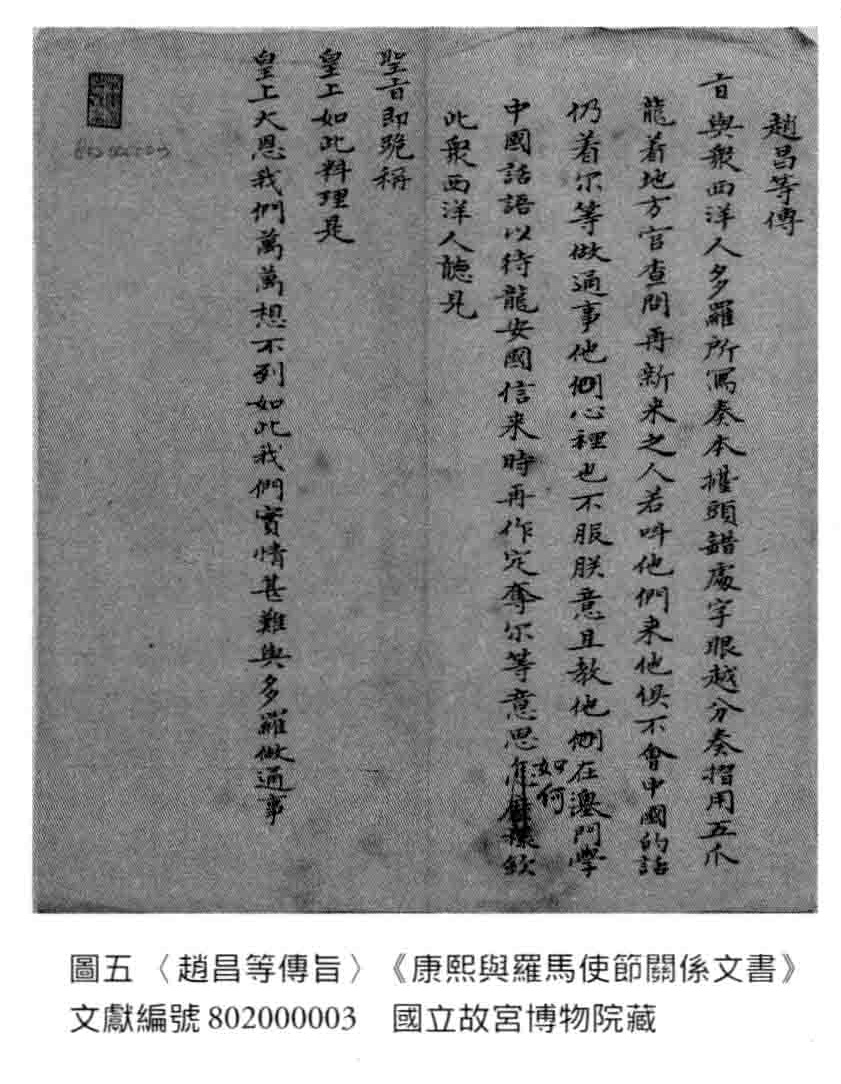
\includegraphics[width=\linewidth,height=.81\textheight,keepaspectratio]{assets/p369-01.jpg}
\end{minipage}
\hfill%
\begin{minipage}[t]{0.479\linewidth}
\vspace{0pt}\setlength{\parindent}{1.5em}
康熙四十九年闰七月十四日，同一天里两广总督赵弘灿上了两个折子，报告西洋来了三位有技艺的人:山遥瞻(GuillaumeBonjour Fabre, 1669-1714)、马国贤(Matteo Ripa,1682-1746)与德理格（TheodoricusPedrini,1671-1746），他们是来查问多罗情况的，然多罗已于五月十二日病故。在两广总督赵弘灿〈奏查问西洋人多罗并进画像等情形〉折中，附有<墨谕〉，其内容与《康熙与罗马使节关系文书》〈赵昌等传谕众西洋人〉（图五）大致同，指责多罗遗折「抬头错处，字眼越分，奏折用五爪龙纹」等种种违例不合中国法

\end{minipage}
\par\addvspace{4pt}

\noindent 制，谕令赵昌、王道化、张常住、李国屏等传旨赵弘灿等，差人查问；至于新到的三位西洋人则奉谕留在广东学习汉话，并等待龙安国讯息传回后再定夺。35

其实这次来华的传教士共六人，除马国贤、德里格、山遥瞻外另有庞克修(Joseph Ceru,1674-1750)、任掌晨(G.Amodei)及潘如(Dominicus Perroni)等，他们都是罗马教廷传信部教士，于康熙四十六年当教皇克莱门十一世听到多罗使华讯息后奉派来华。其中马国贤会画画，德里格长于音律乐器，山遥瞻懂测绘，他们在广东天主堂学了一年汉语，于四十九年十二月到了北京，表达了遵照康熙谕令，奉行利玛窦传教成规，陛见后领取了「永居票」，三人在清宫文化事业中各有表现，且

\vfill
\begin{BookNotes}
\BookNote{33.}{康熙48年7月3日、6日、9月14日李国屏、王道化〈奏报西洋人谢恩折〉、〈奏报西洋人消息未到折〉、〈奏报西洋人情形折〉。}
\BookNote{34.}{详康熙49年2月18日两广总督赵弘灿〈奏进酒洋书信折〉。}
\BookNote{35.}{康熙49年闰7月14日两广总督赵弘灿、广东巡抚范时崇〈奏接到西洋人沙国安来信多罗已故及寄来洋酒事折〉及〈奏查问西洋人多罗并进画像等情形附墨殊批一件〉。}
\end{BookNotes}

% 原图说　图五　〈赵昌等传旨〉　《康熙与罗马使节关系文书》文献编号802000003　国立故宫博物院藏

% 原书第 357 页（PDF 第 370 页）
\BookPage{357}{370}
\noindent 均卒于中国。36

自马国贤等来华以后到康熙五十五年九月康熙发出〈红票〉期间，每届船期康熙皇帝仍旧殷切垂问，令广东具体呈报所到外洋船只数字、国籍及将有技艺才能的西洋人送京，但他得到的消息总是零乱而又不辨真伪的。37例如康熙五十一年(1712)七月十日武英殿监造和素、李国屏奏报，西洋人报艾若瑟仍在罗马；38九月二日和素等再奏：本年洋船带来的讯息，艾若瑟见到了教皇，谈到教内难推行（禁）中国礼；葡萄牙国王于康熙五十年（1711）亦派人向教皇说明，此事（禁约）关系重大，多罗之言不可信等；葡王令驻澳门总督勿听多罗言行事；又报告教皇尚未裁断礼仪问题等。39九月十二日广东巡抚满丕（?-1700）又遣家人转呈了一封教皇函，据满丕奏称：这封信原是教皇带来请多罗转呈皇上的，四十九年七月信抵澳门时，多罗已逝，无人署名送呈，故一直留在澳门；今闻皇上查询有无西洋讯息，因此方由住在澳门西洋教士罗若德送呈，经住广东西洋人庞可秀（P.Jean.Testard，亦译作庞克修）确认为教宗文书。这封信的内容无法得知，康熙看信后即令养心殿拟了一份敕谕，交满丕赶在五十二年（1713）回洋船起航前寄出。40

对康熙而言他派去的人没有回来，寄去的信没有回音，收到的讯息又难辨真伪，因此他在康熙五十五年九月探取了两项更积极的做法：其一令在京的西洋人德理格等依照他的旨意致函教宗41(图六）；德理格与马国贤等即将意旨拟成信函，奉康熙批核后寄给教皇，信中除请教廷派懂得天文、律吕、画工、内外科医术者来华外，也准确表达了康熙极关注的礼仪问题：

\begin{BookQuote}
臣等听得大皇帝旨意云：中国供牌一事并无别意，不过是想念其父母写其名于牌上，以不忘耳，原无写灵魂在其牌上之理。即如尔们画父母之像以存不忘之
\end{BookQuote}

\vfill
\begin{BookNotes}
\BookNote{36.}{详方豪《中国天主教史人物传》第二册〈山遥瞻〉、〈马国贤〉、〈德里格〉。}
\BookNote{37.}{详附表所录康熙50至57年奏折。}
\BookNote{38.}{康熙51年7月10日和素、李国屏奏〈奉谕探报西洋人消息〉。}
\BookNote{39.}{康熙51年9月2日和素、李国屏奏奏报西洋人消息〉。}
\BookNote{40.}{康熙51年9月12日、康熙52年1月10日广东巡抚满丕奏〈奏报进览西洋文书〉及〈奏咨行西洋信函已交付带往折。}
\BookNote{41.}{《康熙与罗马使节关系文书》〈康熙五十五年九月二十九三十日面谕德里格得在京西洋人》802000010。}
\end{BookNotes}

% 原书第 358 页（PDF 第 371 页）
\BookPage{358}{371}
\noindent 意同也。然画像犹恐画工有工拙，不如写其名则无错矣。至于敬天之字，亦不是以天即为天主，乃是举目见天不能见天主；天主所造之物甚多甚大，而在上者莫如天，是以望天存想，内怀其敬耳。其艾若瑟所奉去之旨意乃朕的真旨意。钦此！42 (图七)

\BookArt{p371-01.jpg}{0.990}{0.724}

\vfill
\begin{BookNotes}
\BookNote{42.}{《康熙与罗马使节关系文书》〈德里格、马国贤谨启〉802000011。}
\end{BookNotes}

% 原图说　图六　〈面谕德里格及在京西洋人〉　《康熙与罗马使节关系文书》文献编号802000010　国立故宫博物院藏
% 原图说　图七　〈德里格、马国贤谨启〉　《康熙与罗马使节关系文书》文献编号802000011　国立故宫博物院藏

% 原书第 359 页（PDF 第 372 页）
\BookPage{359}{372}
其二，康熙皇帝让所有来华回国的西洋人成为他的信差，将他的谕旨寄予罗马教廷，此即本文介绍的〈红票〉。本院藏有汉文本〈红票〉底稿，内容与正式发出的印刷本〈红票〉完全相同，唯未塡入使臣「龙安国、薄贤士与艾若瑟、陆若瑟」名字与出洋时间。（图二）这则经康熙皇帝朱笔修改的「廷寄」，当是〈红票〉底稿，并据之译成满文及拉丁文，于康熙五十五年九月十七日由供职内廷十六位西洋人署名，在宫中雕版印制后，经驿道传送广东钤巡抚关防，不封口，交予来华回洋的西洋人带回，这就是〈红票〉的由来。同年九月二十九、三十日，康熙皇帝召见德里格及在京西洋人面谕：只有艾若瑟带回讯息，朕才相信是教化王之意，才决定传教方针。(图六)

根据两广总督杨琳奏，他于康熙五十五年（1716）十月接到由驿站寄来的〈红票〉，即着巡抚用了官防，发与所有洋船上较体面的人带回西洋去了。43这封信终于发生了功能，一年多后陆续传回了康熙皇帝殷切期盼的讯息。

四盼得回音

康熙皇帝大约是在五十七年（1718)夏陆续收到了一些关于〈红票〉及来自教廷的讯息。首先是两广总督杨琳根据新到洋人带来的消息向皇帝奏报了三点：

\begin{BookQuote}
（1）发出的红字票〉在小西洋已有流传，并已带往大西洋；(2)龙安国、薄贤士于四十六年前往大西洋(欧洲）途中遭风难淹毙；（3）艾若瑟、陆若瑟于四十八年抵达大西洋，陆若瑟于五十年身故，艾若瑟目前仍在义大利（大里亚国）。44
\end{BookQuote}

同年七月二十七日杨琳再报:〈红票〉于五十六年十月到达大西洋，教皇已经看到，并已传唤艾若瑟，闻艾若瑟一到罗马便会差来复命。45到了五十九年（1720）六月，艾若瑟果然回到中国，只可惜他在返抵澳门前已逝于船上，将他的灵柩带回来的人是他的徒弟樊守义（1682-1753）。据樊守义供称:他于四十六年随着艾若瑟到了澳

\vfill
\begin{BookNotes}
\BookNote{43.}{康熙57年6月28日两广总督杨琳〈奏报葡英商船到粤并查问回国洋人情形折〉。唯笔者所见两件〈红票〉，均未钤巡抚官防。}
\BookNote{44.}{同上。}
\BookNote{45.}{康熙57年7月27日两广总督杨琳<奏报英法等商船到粤并华侨回籍情形折〉。}
\end{BookNotes}

% 原书第 360 页（PDF 第 373 页）
\BookPage{360}{373}
\noindent 门，次年七月到了欧洲，四十八年二月抵罗马，觐见教皇，报告了多罗使华情形，但教皇对艾若瑟呈文上没有清廷印玺而生疑，命艾若瑟留居国内不准回华。到了康熙五十七年，教皇收到〈红票〉后始准他返回中国。樊守义随艾若瑟到达罗马后便入了耶稣会，追随师父留在义大利修道疏学神学，成为一名司铎。五十八年三月随艾若瑟赴归，临行前教廷国务卿保罗琪枢机（Card.Paulucei,1651-1726）致函艾若瑟，令其以患病为由解释其迟归中国的原因，对于礼仪问题不得作任何解释，以免与教廷禁令抵触；教廷将另遣特使前来阐述。可惜艾若瑟在康熙五十九年二月七日病死归途中，樊守义将其灵柩带回，下葬于澳门；樊守义则经过两广总督杨琳的审询盘查后，连同带回的七箱礼物一并护送进京。樊守义后在北京、山东一带传教，于卒乾隆十八年(1753)。46

\begin{BookQuote}
樊守义返抵国门后不久，康熙五十九年七月二十二日教廷又派来了费理伯
\end{BookQuote}

(Filippo-Maria Cesati,1684-1725)与何济各(OnoratoMaria Ferrari, 1685-1755)两位使者，他们甫抵广东即向两广总督杨琳等表示：教皇所派特使团包括有技艺的人随后即到，并呈上「金线所缝又用金锁封固」的〈表文〉。九月十六日康熙皇帝以费理薄（伯）、何济格（各）二人带来的〈表文〉，未回复艾若瑟传谕，因而拒绝拆阅。47(图八)

康熙皇帝极盼的教廷使臣嘉乐（CarloMezzabarba,1682-1741）于五十九年八月二十七日终于抵达澳门，随行者共二十四人，其中十名拥有特殊技艺，画家二人、音乐家二人、钟表师一人、天文数学家一人、内科与外科各一人、制药师一人、雕刻师一人；他们在广东休息及准备一个月后，于九月二十七日起程赴京。47就在嘉乐使团即将抵京，康熙皇帝在五十九年十一月十八日在乾清宫西暖阁召见西洋人苏霖（Jose Soares,1656-1736)、白晋（JoachimBouvet,1656-1730)、巴多明(Dominique

\vfill
\begin{BookNotes}
\BookNote{46.}{艾若瑟、樊守义事迹，详两广总督杨琳、广东巡抚杨宗仁奏〈奏报樊守义回国并英法船只来粤折〉、〈奏报细问樊守义在西洋情形等折〉、〈奏护送樊守义来京〉及方豪《中国天主教史人物传》第三册，页30-31〈艾若瑟〉、页33-35〈樊守义〉。唯方豪书载，艾、樊二人是与在葡萄牙里斯本出海，葡萄牙国王为艾准备了一艘快船，备有七箱礼物请艾带回呈献皇上；当船行驶到好望角附近艾病逝。据两广总督等奏折录樊守义供词，艾若瑟死亡的地点是在小西洋大狠山地方；所乘船只则是法兰西船。两者稍异，载录供读者参考并待考订。}
\BookNote{47.}{《康熙与罗马使节关系文书》〈养心殿武英殿带西洋人事伊都立等奉旨传谕两广总督广东巡抚》802000007}
\end{BookNotes}

% 原书第 361 页（PDF 第 374 页）
\BookPage{361}{374}
\BookArt{p374-01.jpg}{0.915}{0.388}

\noindent Parrenin,1665-1741)、穆敬远（JoaoMourao,1681-1726)、戴进贤（Ignatius Kgler,1680-1746）、严嘉乐（Mgr. Maigrot de Crissey,1652-1730）、麦大成（Joan FranciscoCardoso,1676-1723)、倪天爵（NicolaqGiampriamo,1686-1759)、汤尙贤(Pierre-Vincent de Tartre,1669-1721)、雷孝思（Jean Baptiste Regis,1663-1736)、冯秉正（J. F.M.A.de Moyriacde Mailla,1669-1748)、马国贤、费隐（Xavier Ehrenbert Fridelli,1673-1743)、罗怀忠(Giovanni Giussepe Costa,1679-1747)、安泰(EtienneRosset,1689-1758)、徐懋德(AndréPereira,1689-1743)、张安多(AntoineMagalhaens,1677-1735)与殷弘绪(FrançoisDentrecolles,1664-1741)等，面谕：

\begin{BookQuote}
倘问及尔等（指嘉乐问话），行教之事，尔众人公（共）同答应，中国行教俱遵利玛窦规矩。48 (图九)
\end{BookQuote}

\vfill
\begin{BookNotes}
\BookNote{48.}{《康熙与罗马使节关系文书》〈康熙五十九年十一月十八日谕西洋人〉802000015。}
\end{BookNotes}

% 原图说　图八　〈养心殿武英殿带西洋人事伊都立等奉旨传谕两广总督广东巡抚〉　《康熙与罗马使节关系文书》文献编号802000007　国立故宫博物院藏

% 原书第 362 页（PDF 第 375 页）
\BookPage{362}{375}
\BookArt{p375-01.jpg}{0.990}{0.661}

\noindent 关于嘉乐使华的经过，前人叙述极多，非本文主题，自不赘述。唯本院藏有〈嘉乐使华日记〉49（图+），详载五十九年十一月二十五日至十二月二十一日康熙皇帝与嘉乐使团交聘与对话细节。根据方豪师考证，该文件于六十年二月康熙皇帝召见使团时交与嘉乐，让他带回转呈教皇；罗马传信部档案处《东方文件》藏有一件，梵蒂冈图书馆另藏两件。仅就〈嘉乐使华日记〉重要内容摘录如下：

\vfill
\begin{BookNotes}
\BookNote{49.}{据方豪考证《记记在有康燕60年2月召见嘉乐时曾交与嘉乐，让他带回转呈教皇。罗马传信部档案处}
\end{BookNotes}

% 原图说　图九　〈康熙五十九年十一月十八日面谕西洋人等〉　《康熙与罗马使节关系文书》802000015　国立故宫博物院藏

% 原书第 363 页（PDF 第 376 页）
\BookPage{363}{376}
\BookArt{p376-01.jpg}{0.990}{0.594}

\noindent 五十九年十一月二十六日令伊都立、赵昌等传旨查询来使目的，嘉乐答称有二：（1）求中国大皇帝俯赐允准着臣管在中国传教之众西洋人；（2）求中国大皇帝俯赐允准着中国入教之人俱依前岁教王发来条约（禁约）内禁止之事。

二十七日伊都立、赵昌等传旨嘉乐，尔教王所求之事，朕俱俯赐允准。但尔教王条约与中国大道理大相悖戾，尔天主教在中国行不得，务必禁止。教既不行，在中国传教之西洋人亦属无用，除会技艺的留用，再年老有病不能回去者仍准存留，其余在


% 原图说　图十　〈嘉乐使华日记〉　《康熙与罗马使节关系文书》文献编号802000005（局部）　国立故宫博物院藏

% 原书第 364 页（PDF 第 377 页）
\BookPage{364}{377}
\noindent 中国传教之西洋人俱带回西洋。且尔教约只可禁止尔西洋人，中国人非尔教王所可禁止。其准留之西洋人可依约自行修道，不许传教。此即准尔教王所求二事。嘉乐接旨后答称待祈祷蒙主指示后再回奏。

二十八日传旨嘉乐，朕之旨意前后无二，尔教王条约（禁约）与中国道理大相悖谬，教王表章，朕亦不览。尔即回去，西洋人中不会技艺者，尔俱带回。尔带来会技艺之九人，愿效力者留用，不愿在中国者，即同回去。嘉乐恳请候至明年开河时由水路返回广东。

二十九日传旨嘉乐，尔西洋人不通中国诗书，不解中国文义，如何妄辨中国道理。嘉乐恳请皇上赐览教王〈表章〉及〈禁约〉，其中有合中国道理者，求准入教者依行；有不合道理者，请明示，嘉乐能改者即改，不能改者，即明白寄字转达教王。康熙同意览表及禁约，并传旨嘉乐等移居五阿哥房内。

十二月一日传旨嘉乐，令于后日陛见，并准许与在京西洋人见面。

三日康熙御九经三事殿筵宴嘉乐，亲接〈表文〉。赐克食，酒一爵后问嘉乐:「朕览西洋图画内有生羽翼之人，是何道理？」嘉乐奏云:「寓意天神灵速如有羽翼非真有生羽翼之人。」上谕：「中国人不解西洋字义，故不便辨尔西洋事理；尔西洋人不解中国字义，如何妄论中国道理之是非，朕问此即此意也。」赐嘉乐貂褂一件。

五六七日互献贡物、礼物。

十二日传旨嘉乐，先差回西洋之人，应起程，迟则赶不上二月回小西洋船了。


% 原书第 365 页（PDF 第 378 页）
\BookPage{365}{378}
\noindent 十三日上于清西书屋召见嘉乐及众西洋人，令于随行人中选择两名回罗马去传谕朕旨：（1）教王遣使谢恩，朕深加念；（2）教王遣尔请安，朕躬康建；（3）教王贡物朕念远人胥服之情，俯赐存留。

十七日上于渊鉴斋召见嘉乐及带来、原在京之西洋人，再辩中国礼仪，重申：「欲议论中国道理，必深通中国文理，读尽中国诗书，方可辩（原作辨）论。朕不识西洋之字，所以不论西洋事。利玛窦来中国传教，有何不合尔教之处？」嘉乐答：「如供牌位、称天，即不合教。」康熙答：「供牌位，为后人尊敬之意；呼天为上帝，即如称朕为万岁、称朕为皇上，称呼虽异，敬君之心则一。嘉乐哀恳道:「教王不许臣辩（辨）论中国道理，臣亦不敢辩（辨）论。」

十八日先遣回洋二人由驿道送出，嘉乐致教王信函交旧西洋人译出呈览过寄出。

二十一日译出汉字教王〈禁约〉（即《康熙与罗马使节关系文书》）呈览，朱批：「览此条约，只可说得西洋人等，小人如何言得中国之大理…以后不必西洋人在国行教，禁止可也。」嘉乐闻旨，即表示来时教王交付「条约（禁约）解说」一张，恳请皇上赐览。案：笔者以为「条约（禁约）解说」一张，应即为〈八项特准〉:（1）准许教徒家中供奉祖宗牌位；（2）准许中国教徒对亡人的礼节；（3）准许非宗教性的敬孔典礼；（4）准许在改正的牌位前或亡人前叩头；（5）准许在葬礼中焚香点烛；（6）准许在改正的牌位前或亡人棺木前供陈果蔬；（7）准许新年和其他节日在改正牌位前叩头；（8）准许在改正的牌位前，焚香点烛，在墓前供陈果蔬。虽然在「特准」之后有些规范，例如牌位上只许写父母名字，两旁加注天主


% 原书第 366 页（PDF 第 379 页）
\BookPage{366}{379}
教孝敬父母的道理，所有礼节声明不从俗迷信，只遵行社会俗礼等。50基本上是依照康熙的旨意，对教皇「禁约」作了极大的修正与解释。

二十二日

译出教王〈条约解说〉呈览；朱批：「此数条解说均为当日严珰在御前辩过的」。极严厉批判〈禁约〉，又重申中国道理。

案：基本上从御览过〈条约解说〉后，康熙对嘉乐的态度逐渐改善，两天后宽恕了严珰、德里格等的罪。

二十三日

于清溪书屋召见嘉乐及众西洋人，传谕:「尔西洋人自己流入异端之处，自己不

自知，反指中国道理为异端。及至辩论之际，一字又不能回答…」

二十四日

于清溪书屋召见嘉乐及众西洋人传谕:「经尔等再三哀恳，朕将严珰、德里格等之事从宽不究。」

嘉乐则表达待自己回洋定将皇上旨意向教王解释明白。

「目今节近，尔于明岁再定回去日期。今事体俱已明白，朕之旨意尔亦全晓，雨是使臣，辩论道理时，朕必直言无隐，尔既不复争辩，朕仍前优待。朕原视中外为一家，不分彼此，尔可少息一二日，京城内天主堂随尔便居住，以副朕怀柔至意，钦此。」《康熙与罗马使节关系文书》所载嘉乐使华日记到此日止，据方豪在梵蒂冈图书馆所见两份日记，一止于康熙六十年（1721）正月初五日，详载嘉乐于十二月二十九、三十（除夕）、正月初一日，进宫赐宴及拜年情形；一止于正月二十八日禀文及二月二十三日到省，继续记载嘉乐入宫过年赐宴乐情形及赴归赐礼品等事。51康熙于六十年二月初四以隆重的礼仪接见了嘉乐的辞行，二月初六离京，四月十四日到广东，四

\vfill
\begin{BookNotes}
\BookNote{50.}{案嘉乐使华期间曾针对教廷〈禁约〉拟定了〈八项特许〉，至于何时公布〈八项特许〉则各人研究不同。笔者以为：嘉乐此时出示的「条约（禁约）解说」，即是〈八项特许〉」；再分析〈八项特许〉，不难发现其内容深受康熙辩论中国礼仪的影响；再者《八项特许》是针对《禁约》中的祭孔、敬祖、丧葬习俗作出让步与通容。自「条约（禁约）解说」呈览后康熙的态度亦趋缓和。}
\BookNote{51.}{详方豪《中国天主教人物传》第二册，页326-342，〈嘉乐〉。}
\end{BookNotes}

% 原书第 367 页（PDF 第 380 页）
\BookPage{367}{380}
\noindent 月二十八日抵澳门，至十月二十一日带着多罗灵柩返航罗马。嘉乐回罗马后升为枢机主教，至乾隆六年（1741）卒。52

从上述交聘过程中，可知康熙皇帝并未反对天主教在中国传播，他所坚持的是要按他的规矩传教；他以极大的宽容传谕多罗、嘉乐，反复申论中国礼仪不是迷信，与天主教教义没有抵触，并努力建立与教廷沟通的管道，以各种方式传信教廷，当嘉乐不再申辩并宣布八项特许〉后，康熙朝皇权与教权之争也告落幕。

\BookSubheading{结论}

\begin{BookQuote}
红票〉与本院所藏《康熙与罗马使节关系文书》以及内务府官员和两广总督巡
\end{BookQuote}

抚的各相关奏折，记录了一段已广为人知的中梵关系史，本文旨在介绍档案，并说明康熙皇帝从未反对天主教在华传播。康熙皇帝在康熙三十一年所颁布的〈宽容敕谕〉（图+一），成为十九世纪中叶以前承认天主教自由传教的法定文件。53可惜十八世纪初罗马教廷改变了利玛窦以来尊重中国礼俗的传教方式，引发了康熙朝礼仪之争，也改变了中梵关系的发展。档案中所见康熙皇帝以极大的耐心与宽容一再传谕，反复申论中国礼仪不是迷信，与天主教教义没有抵触，并努力打通与教廷沟通的直接管道。〈红票〉的广为传布，是康熙皇帝想出来的传信方法，成为一件非常特殊的清代档案。康熙皇帝虽坚持西洋传教士必须遵守大清法度在华传教，但终其一生始终未禁天主教，领有「票」的传教士是可以传教的。根据《总管内务府档案》，康熙四十七年领票传教的西洋人达六十四人，分布陕西、山西、直隶、山东、湖广、江西、贵州、浙江、江苏、广东等各地。54康熙皇帝传谕鼓励西洋传教士领票，并安慰已领票者：

\vfill
\begin{BookNotes}
\BookNote{52.}{详顾卫民《中国与罗马教廷关系史略》，页81-82。}
\BookNote{53.}{康熙31年2月初5日，清圣祖应钦天监徐日升（ThomasPereira)、安多（AntoniusThomas）奏请，开放教禁。上谕曰：「西洋人并无为恶作乱之处，又并非左道惑众异端生事。喇嘛僧道等等，庙尚容人烧香行走，西洋人并无违法之事，及行禁止，似属不宜，相应将各处天主堂俱照旧存留，凡进香供奉之人，仍文许照常行走，不必禁止。俟命下之日，随行直隶各省可也。」见「军机处月折包」048450号，〈抄写得西洋堂内康熙31年碑文〉。}
\BookNote{54.}{详见高振田〈康熙帝与西洋传教士〉及陈莉婷《从容教到禁教：清朝政府对天主教政策的转变1644-1820》，国立台湾师范大学历史学研究所硕士论文，2000年。}
\end{BookNotes}

% 原书第 368 页（PDF 第 381 页）
\BookPage{368}{381}
\BookArt{p381-01.jpg}{0.990}{0.485}

\noindent 教化王若再怪你们遵利玛窦不依教化王的话，教你们回西洋去，朕不教你们回去；倘教化王听了多罗的话，说你们不遵教化王的话，得罪天主，必定教你们回去，那时朕自然有话说，说你们在中国年久，服朕水土，就如中国人一样，必不肯打发回去。…你们领过票的，就如中国人一样，尔等放心，不要害怕领票。55(图十二)

康熙五十四年，直隶省领票西洋人与民众起了纷争，康熙皇帝下达维护西洋传教士的谕旨：近日闻得京中西洋人说，真定府内有票西洋人，偶有比（彼）此争地，以致生祸授打等语，未知虚实，但西洋人到中国将三百年，未见不好处，若事无大关，从宽亦可，尔细察缘由情形，写折奏闻。（图十三)

\vfill
\begin{BookNotes}
\BookNote{55.}{《康熙与罗马使节关系文书》〈谕孟由义等众西洋人〉802000002。}
\end{BookNotes}

% 原图说　图十一　康熙三十一年〈宽容敕谕〉抄件　文献编号048450　国立故宫博物院藏

% 原书第 369 页（PDF 第 382 页）
\BookPage{369}{382}
\BookArt{p382-01.jpg}{0.990}{0.422}

\noindent 正因「西洋人到中国将三百年，未见不好」，发生礼仪之争时正当康熙皇帝令西洋传教士绘制《皇舆全览图》时期，康熙皇帝对西方科学的热情与喜爱，完全折射到中梵交聘过程中对多罗及教廷的惊人耐性与宽仁，他站在前线，反复申辩，积极沟通，留下了大量档案，让后人对清圣祖康熙皇帝有更深入的了解。


% 原图说　图十二　〈谕西洋人〉　《康熙与罗马使节关系文书》文献编号802000002　国立故宫博物院藏
% 原图说　图十三　直隶总督赵弘灿奏折附件〈朱批〉文献编号401000971　国立故宫博物院藏

% 原书第 370 页（PDF 第 383 页）
\BookPage{370}{383}
\BookArt{p383-01.jpg}{0.990}{0.830}


% 原图说　本文征引满汉文奏折出处
